% ------------------------------------------------------------------------
% ------------------------------------------------------------------------
% abnTeX2: Modelo de Trabalho Academico (tese de doutorado, dissertacao de
% mestrado e trabalhos monograficos em geral) em conformidade com 
% ABNT NBR 14724:2011: Informacao e documentacao - Trabalhos academicos -
% Apresentacao
% ------------------------------------------------------------------------
% ------------------------------------------------------------------------


\documentclass[
	% -- opções da classe memoir --
	12pt,				% tamanho da fonte
	openright,			% capítulos começam em pág ímpar (insere página vazia caso preciso)
	%twoside,			% para impressão em verso e anverso. Oposto a oneside
	oneside,
	a4paper,			% tamanho do papel. 
	% -- opções da classe abntex2 --
	%chapter=TITLE,		% títulos de capítulos convertidos em letras maiúsculas
	%section=TITLE,		% títulos de seções convertidos em letras maiúsculas
	%subsection=TITLE,	% títulos de subseções convertidos em letras maiúsculas
	%subsubsection=TITLE,% títulos de subsubseções convertidos em letras maiúsculas
	% -- opções do pacote babel --
	english,			% idioma adicional para hifenização
	french,				% idioma adicional para hifenização
	spanish,			% idioma adicional para hifenização
	brazil				% o último idioma é o principal do documento
	]{abntex2}

% ---
% Pacotes básicos 
% ---
\usepackage{lmodern}			% Usa a fonte Latin Modern				
\usepackage[T1]{fontenc}		% Selecao de codigos de fonte.
\usepackage[utf8]{inputenc}		% Codificacao do documento (conversão automática dos acentos)
\usepackage{lastpage}			% Usado pela Ficha catalográfica
\usepackage{indentfirst}		% Indenta o primeiro parágrafo de cada seção.
\usepackage{color}				% Controle das cores
\usepackage{graphicx}			% Inclusão de gráficos
\usepackage{microtype} 			% para melhorias de justificação
\usepackage[font={small,it}]{caption}

% ---
		
% ---
% Pacotes adicionais, usados apenas no âmbito do Modelo Canônico do abnteX2
% ---
\usepackage{lipsum}				% para geração de dummy text
% ---

% ---
% Pacotes de citações
% ---
\usepackage[brazilian,hyperpageref]{backref}	 % Paginas com as citações na bibl
\usepackage[alf]{abntex2cite}	% Citações padrão ABNT

% define o caminho das imagens
\graphicspath{{Imagens/}}

% --- 
% CONFIGURAÇÕES DE PACOTES
% --- 

% ---
% Configurações do pacote backref
% Usado sem a opção hyperpageref de backref
\renewcommand{\backrefpagesname}{Citado na (s) página (s) :~}
% Texto padrão antes do número das páginas
\renewcommand{\backref}{}
% Define os textos da citação:
\renewcommand*{\backrefalt}[4]{
	\ifcase #1 %
		Nenhuma citação no texto.%
	\or
		Citado na página #2.%
	\else
		Citado #1 vezes nas páginas #2.%
	\fi}%
% ---

\newcommand{\monoTitulo}{Utilização de Clusterização Fuzzy e Redes Neurais Artificiais para Prevenção de Intrusao} 
\newcommand{\monoIDS}{\textit{Intrusion Detection System} } 
\newcommand{\monoIPS}{\textit{Intrusion Prevention System} }
\newcommand{\monoFireWall}{\textit{firewall}}




% ---
% Informações de dados para CAPA e FOLHA DE ROSTO
% ---
\titulo{\monoTitulo}
\autor{Lucas Teles Agostinho \\ Rodrigo Mendonça da Paixão}
\local{São Paulo -- Brasil}
\data{2017}
\orientador{Eduardo Heredia}
%\coorientador{Nome Completo}
\instituicao{%
  Centro Universitário Senac
  \par
  Bacharelado em Ciência da Computação
}
\tipotrabalho{Monografia (Graduação)}

% ---
% Configurações de aparência do PDF final

% alterando o aspecto da cor azul
\definecolor{blue}{RGB}{41,5,195}

% informações do PDF
\makeatletter
\hypersetup{
     	%pagebackref=true,
		pdftitle={\@title}, 
		pdfauthor={\@author},
    	pdfsubject={\imprimirpreambulo},
	    pdfcreator={LaTeX with abnTeX2},
		pdfkeywords={abnt}{latex}{abntex}{abntex2}{trabalho acadêmico}, 
		colorlinks=true,       		% false: boxed links; true: colored links
    	linkcolor=blue,          	% color of internal links
    	citecolor=blue,        		% color of links to bibliography
    	filecolor=magenta,      		% color of file links
		urlcolor=blue,
		bookmarksdepth=4
}
\makeatother
% --- 

% --- 
% Espaçamentos entre linhas e parágrafos 
% --- 

% O tamanho do parágrafo é dado por:
\setlength{\parindent}{1.3cm}

% Controle do espaçamento entre um parágrafo e outro:
\setlength{\parskip}{0.2cm}  % tente também \onelineskip

% ---
% compila o indice
% ---
\makeindex
% ---

% ----
% Início do documento
% ----
\begin{document}


% Retira espaço extra obsoleto entre as frases.
\frenchspacing 

% ----------------------------------------------------------
% ELEMENTOS PRÉ-TEXTUAIS
% ----------------------------------------------------------
% \pretextual

% ---
% Capa
% ---
\imprimircapa
% ---

% ---
% Folha de rosto
% (o * indica que haverá a ficha bibliográfica)
% ---
\imprimirfolhaderosto%*
% ---

% ---
% RESUMOS
% ---

% resumo em português
\setlength{\absparsep}{18pt} % ajusta o espaçamento dos parágrafos do resumo
%\begin{resumo}

   
 %\textbf{Palavras-chaves}: IDS,Rede,Internet
%\end{resumo}

% ---
% inserir lista de ilustrações (figuras)
% ---
%\pdfbookmark[0]{\listfigurename}{lof}
%\listoffigures*
%\cleardoublepage
% ---

% ---
% inserir lista de tabelas
% ---
%\pdfbookmark[0]{\listtablename}{lot}
%\listoftables*
%\cleardoublepage
% ---

% ---
% inserir lista de abreviaturas e siglas
% ---
\begin{siglas}
  \item[AG] Algoritmos Genéticos
  \item[API] Application Programming Interface
  \item[IA] Inteligência Artificial
  \item[CPU] Central Processing Unit
  \item[PCV] Problema do Caixeiro Viajante
  \item[PRV] Problema de Roteirização de Veículos
  \item[PRVJT] Problema de Roteirização de Veículos com Janela de Tempo
  \item[TS] Têmpera Simulada
\end{siglas}
% ---

% ---
% inserir o sumario
% ---
\pdfbookmark[0]{\contentsname}{toc}
\tableofcontents*
\cleardoublepage
% ---

% ----------------------------------------------------------
% ELEMENTOS TEXTUAIS 
% ----------------------------------------------------------
\textual

% ----------------------------------------------------------
% Capitulo 1
% ----------------------------------------------------------

\chapter[Introdução]{Introdução}
%\addcontentsline{toc}{chapter}{Introdução}
% ----------------------------------------------------------

\section{Motivação}

No meio empresarial é essencial pensar na área logística, essa é a área que gerencia os recursos,
matérias-primas, componentes, equipamentos, serviços e informação necessária para execução e 
controle das atividades da empresa. Ela tem como foco orquestrar estes itens de forma a encontrar
a melhor condição de operação no menor tempo possível~\cite{DIAS}.

Um dos principais pontos dentro da logística é o transporte, onde chega a custar até 60% 
de seu custo total.\cite{RODRIGUES} Logo é de interesse das empresas conseguir minimizar o custo de escoamento de seus produtos.

Graças a sua importância no processo produtivo a logística se tornou um grande fator competitivo entre empresas.
Isso se deve ao fato que a cadeia de suprimento está relacionada com agregação de valores e disponibilidade dos seus bens e
serviços para os clientes, fornecedores da empresa e os demais interessados. Independe do lugar que o interessado esteja um serviço ou produto apenas tem valor quando 
ele está disponível para ser consumindo~\cite{TSUDA}.

No planejamento estratégico de logística o principal problema esta relacionado a roteirização de veículos~\cite{TSUDA} também conhecido como PRV, 
para encontrar a rota menos custosa, é necessário calcular as possíveis combinações de um determinado problema. Contudo, dependendo do numero de combinações pode requerer um
processamento muito elevado, levando muito tempo para encontrar a solução ótima. Esse problema se encaixa na categoria NP-Difícil~\cite{CUNHA}, Neste tipo de problema não existe
uma nenhum algoritmo conhecido que consiga resolvê-lo em tempo polinomial.

\section{Objetivos}

Desenvolver uma solução que resolva o problema de PRV utilizando a meta-heurística algoritmos genéticos. Um sistema capaz de calcular uma rota entre vários destinos 
levando em consideração restrições de tempo e notificando a quantidade de motoristas necessários para realizar todas as entregas ate uma data limite estipulada. Além de levar  
em consideração o tempo de transito entre estes pontos, permitindo que um motorista possa recalcular a sua rota para otimizar o tempo a qualquer momento.

\subsection{Objetivos Específicos}

Utilizar uma API de terceiros para adquirir informações sobre endereços ou pontos no mapa, alem do tempo de locomoção entre os pontos.
Implementar um algorítimo genético capas de minimizar a rota entre todos os pontos.
Introduzir janelas de tempo nas entregas e adaptar o algoritmo genético para levar essas janelas de tempo em consideração.
Definir fata/hora limite e dividir entrega em mais de um entregador para respeitar essa hora/data limite caso seja necessário.
Criar um aplicativo capaz de consultar e recalcular a rota.

\section{Método de trabalho}

Desenvolver uma implementação de algoritmos genéticos capaz de calcular rotas entre pontos geográficos.
Desenvolver uma aplicação Web capaz de receber uma quantidade N de pontos no mapa uma data limite, e a partir deles utilizar a implementação previa para calcular as rotas e 
notificar o utilizador.
Ter uma pagina onde um motorista possa recalcular sua rota em qualquer ponto.

\section{Organização do trabalho}
Este trabalho é dividido em 4 capítulos. O primeiro capitulo faz uma introdução geral do problema, descrever os objetivos e a motivação para a resolução do problema proposto.

O segundo capitulo trata do problema de forma separada, mostrando o que existe na literatura para uma possível solução. Também explica de forma mais detalhada o funcionamento de dois exemplos de busca heurística, demostrando uma aplicação em um trabalho da literatura e dos algoritmos genéticos, explicando seu funcionamento e aplicação na literatura.
O terceiro capitulo é a proposta apresentada para a criação deste trabalho.



% ----------------------------------------------------------
% Capitulo 2
% ----------------------------------------------------------
\chapter[Revisão de Literatura]{Revisão de Literatura}

%\addcontentsline{toc}{chapter}{Revisão de Literatura}
% ----------------------------------------------------------

\section{Busca de caminhos}

\subsection{O Algoritmo A*}

O algorítimo A* é um dos mais populares soluções no ramo de busca de caminhos, o algoritmo garante achar o menor caminho entre dois pontos \cite{PEHart}, porem gera uma grande arvore de busca nos processos, consumindo muito tempo e memoria, é comum haver modificações no algorítimo para explorar uma arvore de busca menor, diminuindo o tempo para achar um caminho sacrificando a garantia de se encontrar o melhor caminho no final. \cite{Botea}.

O algoritmo A* em sua forma tradicional, utiliza a formula heurística f(n) = g(n) + h(n), onde g(n) é o custo para chegar ao nó n, e h(n) é o custo estimado para atingir o nó de destino a partir do nó n. Este sempre deve ser menor ou igual a distancia real entre o ponto n e o destino. Para cada iteração sobre os vizinhos do nó atual é calculado o f(n) e adicionado em uma lista de nós abertos (A), mantendo uma referencia do no que serviu de origem para chegar nele, caso o nó ja esteja na lista e o valor de f(n) novo for menor, o valor de f(n) e o nó de origem é substituído pelo novo. Depois é verificado na lista o menor valor de f(n), este é removido, adicionado a lista de nos fechados (F) e a partir desse ponto, ele se torna o nó atual, quando o nó atual é o mesmo nó de destino o algorítimo retorna o caminho encontrado, assim podemos encontrar a solução ideal. \cite{PEHart}

Podemos aplicar o algoritmo A* em um Grafo direcionado ponderado por exemplo. (Figura 1)


\begin{minipage}{\linewidth}
    \makebox[\linewidth]{
        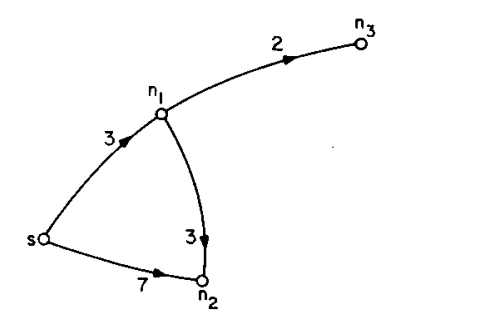
\includegraphics[keepaspectratio=true,scale=0.5]{ibagens/figura1.png}}
    \captionof{figure}{Grafo para busca \cite{PEHart}}
\end{minipage}


\begin{description}
    \item[Figura 1] Consiste em um nó inicial s e mais três outros nós (n1,n2,n3). As arestas contem a direção e o custo do trajeto. Se partirmos do algorítimo A* para produzir um subgrafo do melhor caminho, partindo de s podemos ir para n1 e n2, os valores de g(n1) e g(n2) são respectivamente 3 e 7. Supondo que A* expanda n1, sucedido por n2 e n3, nesse ponto g(n3)=3+2=5,o valor de g(n2) é diminuído pois um caminho de menor custo foi encontrado  3+3=6, o valor de g(n1) continua sendo 3. 
    O próximo passo seria estimar o h(n), podem essa função vai depender muito do domínio do problema, muitos problemas de encontrar o menor caminho entre dois pontos de um grafo possuem alguma "informação física" que pode ser usada de alguma forma para estimar o h(n), podemos em nosso exemplo, se definirmos como cidades ligadas por estradas, h(n) poderia ser a distancia aérea da cidade n até a cidade objetivo, essa distancia seria menor do que qualquer estrada da cidade n até o objetivo \cite{PEHart}. Em jogos digitais e buscas em tempo real é muito comum trabalhar em cima de mapas em forma de matrizes bidimensionais, esse sera o foco dos algoritmos que trataremos, nesses casos fica simples tratarmos o h(n) com a distancia euclideana ou manhatam entre n e o destino. \cite{Yngvi}
\end{description}

Quando definimos o mapa de busca em uma matriz bidimensional NxM, situação comum em jogos digitais e problemas de busca em tempo real \cite{Ross_Graham} \cite{Ulysses} precisamos definir os custos de movimentação entre os vizinhos do ponto n, e a função heurisca h(n). O custo de movimentação na grade pode variar basicamente em dois tipos, levando as diagonais em consideração ou não.

O modelo em \textit{tile}, onde o movimento do agente está restrito aa quatro direções ortogonais com custo 1, e \textit{octile}, onde o agente pode ainda mover-se na diagonal com custo equivalente ao valor da hipotenusa de um triangulo retângulo com catetos igual a 1, sendo assim  $ \sqrt{2}  \approx 1.4 $. É comum para fim de simplificar os cálculos multiplicar os valores de custo por 10 ou 100 como pode ser visto na figura 2.

\begin{minipage}{\linewidth}
    \makebox[\linewidth]{
        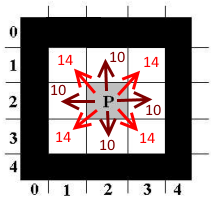
\includegraphics[keepaspectratio=true,scale=1.5]{ibagens/mov_cost.png}}
    \captionof{figure}{Custo de movimentação}
\end{minipage}

Uma limitação do A*, é o fato que ele requer uma grande quantidade de recursos da CPU, caso haja muitos nós a pesquisar como é o caso em grandes mapas que sãp populares em jogos recentes, isso  pode causar pequenos atrasos.
Esse atraso pode ser agravado caso haja múltiplos agentes IA ou quando o agente tem que se mover de um lado do mapa para o outro 

Este alto custo de recursos da CPU pode fazer com que o jogo congele até que o caminho ideal seja encontrado. Game designers tentam superar esses problemas realizando ajustes nos jogos, de forma a tentar evitar estas situações \cite{Timothy}.

Podemos observar o motivo do alto custo, a heurística fornece uma expansão considerável dos nós, que são mantidos na memoria durante todo o processamento. (Figura 3)

\begin{minipage}{\linewidth}
    \makebox[\linewidth]{
        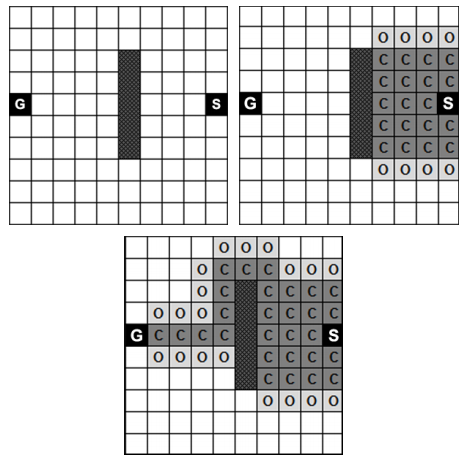
\includegraphics[keepaspectratio=true,scale=1]{ibagens/figura2.png}}
    \captionof{figure}{Exemplo de A* \cite{Ulysses} }
\end{minipage}

\subsection{Aplicações}
Aplicações para os algoritmos de busca podem ser diversos, como por exemplo, em um simulador de carro corrida \cite{JungTing}. Utilizando o algoritmo do A* com duas modificações para encontrar o melhor caminho enquanto evita os obstáculos entre o ponto de inicio e o ponto de destino. 
A primeira modificação consiste em utilizar o Teorema de Triângulos de Pytagoras, onde primeira calcula a distancia entre dois pontos(1 e 2), verifica se existe algum obstaculo dentre eles, se existir, utiliza o terceiro ponto para calcular a Hipotenusa e verifica se existe obstaculo entre a hipotenusa, se não existir, remove o ponto 2 e começa a considerar o caminho do ponto 1 para o ponto 3. A segunda modificação consiste em somente ir para frente, isso significa, procura somente os pontos a frente do carro, direita, esquerda e frente, simulando um controle de carro.

O projeto utiliza 3 pistas reais de corrida da Formula 1, Peru, Itália e Hungria, sendo cada pista, uma imagem de escala 1280x782 pixels retiradas do site oficial da Formula 1. O Carro é implementado em Microsoft XNA Game Studio, plataforma usada para desenvolver jogos para Windows Phone, Xbox e Windows. As Imagens das pistas são modificadas para serem mapas de detecção de colisão, a pista é pintada de preto, indicando onde o carro pode andar e o resto pintado de branco indicando os o carro não pode andar. O carro tem o tamanho de 18x12 pixels e uma movimentação de 2 pixels por segundo. Como o XNA trabalha com uma taxa de quadros de 60 quadros por segundo, o carro se movimenta a 120 pixels por segundo.

Os resultados da primeira modificação conseguiu economizar ciclos de CPU, reduzindo o numero de pontos indicadores da pista em 97\%. A segunda modificação tem a vantagem de obter o tempo de volta mais curto, por que reduz o numero de nós do algoritmo A* de 4 para 3 nós]. A desvantagem é que o carro pode balançar em curvas acentuadas. Em geral, as modificações garantiram uma melhoria em performance, economizando o numero de ciclos de CPU.

\section{Algorítimos genéticos}


\subsection{Aplicações}
Existem vários aplicações para os algoritmo geneticos, por serem uma inteligencia artificial não supervisionada, de rápido aprendizado e podendo ser paralelizado.

O modelo m-PRC(Problema de Rotas de Cobertura multi-veiculo) é uma aplicação de algoritmos geneticos para construção de rotas em uma região mapeada, para encontrar uma boa distribuição de viaturas para patrulhamento urbano usado por departamentos de segurando como a policia, guardas municipais ou segurança privada. 
O Modelo é definido como um grafo G=(V U W, E) não direcionado, onde V U W compõem o conjunto de vértices e E o conjunto de arestas, ou seja, o subgrafo induzido por E e um grafo completo cujo conjunto de nós é V. 
V são todos os vértices que podem ser visitados e é composto pelo subconjunto T, que são os vértices que devem ser visitados por algum veiculo. W é um conjunto de vértices onde todos os M veículos devem passar. M é o numero de rotas de veículos que começam no vértice base V0. O m-PRC atribui o conjunto de m rotas de veículos com as restrições: Todas as m rotas de veículos começam e terminam na base V0, Tem exatamente m rotas, Cada vértice de V pertence a no máximo uma rota, Cada vértice de T pertence a exatamente uma rota, com exceção a base, Cada vértice de W deve ter uma rota que passa por ele e em uma distancia C de um vértice V visitado, O modulo da diferença entre o número de vértices de diferentes rotas não pode exceder um determinado valor R.

\begin{minipage}{\linewidth}
	\makebox[\linewidth]{
		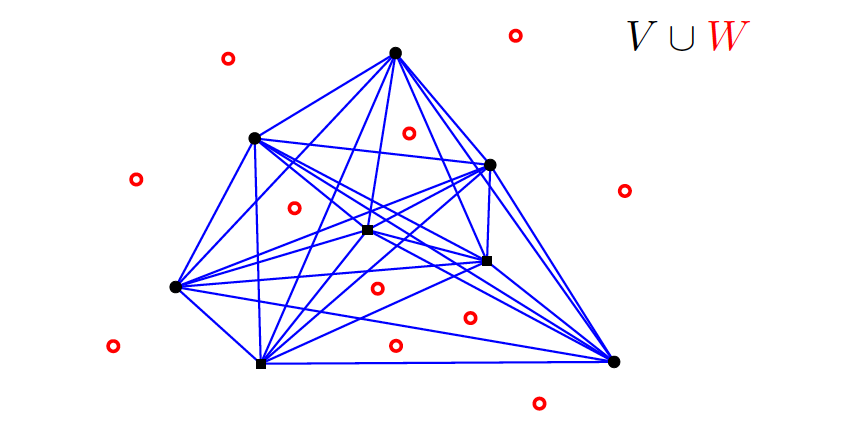
\includegraphics[keepaspectratio=true,scale=0.5]{ibagens/grafoMPRC.png}}
	\captionof{figure}{Exemplo de gráfo não direcionado para V U W. \cite{Washington} }
\end{minipage}



\section{Algoritmos de busca paralelo}

\section{Algorítimos genéticos para busca de caminhos}
Buscando melhorar a eficiência dos algoritmos de busca, foram criadas formas hibridas, levando os algoritmos genéticos analisarem todo o percusso,ajudando o algoritmo de busca em momentos que a próxima ação é incerta.

Utilizando o algoritmo de busca BFS (\textit{Best First Search}), foi desenvolvido o modelo PPGA (\textit{Patterned based Pathfinding with Genetic Algorithm}). O modelo utiliza algoritmos genéticos como um modulo para calcular os sub caminhos ao longo do processo de busca, cada vez que o modulo é chamado, herda informações da chamada anterior, tendo um ganha considerado de desempenho. O modulo é chamado, quando nenhum dos valores dados pelo BFS são melhores que o valor atual. Os resultados da analise do PPGA foram bons, por encontrar boas soluções em um curto período de tempo, mostrando ser muito bom para mapas onde o percurso segue um padrão, mas perdendo para o BFS para mapas mistos ou que não seguem o mesmo padrão ao longo o percurso, considerando o modelo como promissor, indicando que mudanças nos parâmetros do algoritmo genéticos, pode melhorar o desempenho dos testes \cite{Ulysses}.

\begin{minipage}{\linewidth}
	\makebox[\linewidth]{
		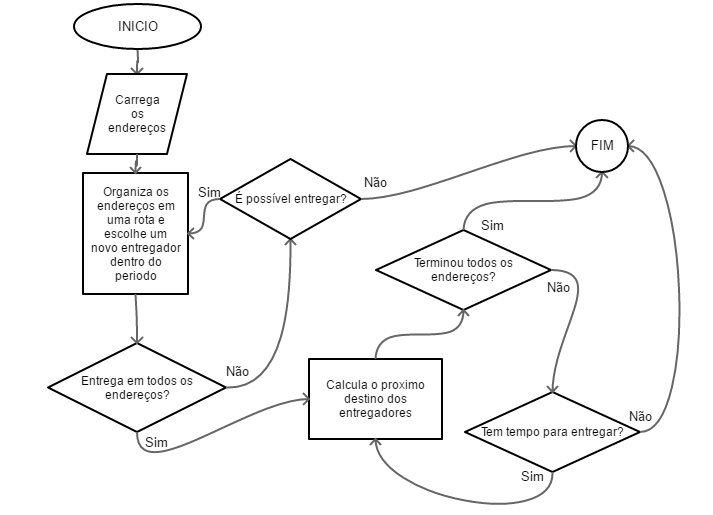
\includegraphics[keepaspectratio=true,scale=0.5]{ibagens/Fluxograma.png}}
	\captionof{figure}{Fluxograma do Modelo \cite{Ulysses} }
\end{minipage}

O modelo GAMMA(\textit{Genetic Algoritmo Manufactured Maneuvering Algorithm}), consiste em uma modificação do A* de forma que o caminho total é separado em caminhos mais curto. O algoritmo prepara o primeiro caminho e calcula o caminho mais curto entre eles, a posição final do resultado é usada como inicial para o próximo calculo, com isso, permitindo que o modelo GAMMA procure caminhos em tempo real por que se o caminho for alterado a sua leitura é parcial do caminho completo.\cite{Ryan}



\section{Algorítimos genéticos paralelos ou distribuídos para busca de caminhos}

Foi demonstrado que algoritmos genéticos paralelos são eficientes para a resolução de problemas de busca de caminho, tal como o clássico problema do caixeiro viajante, que consiste em dado um numero finito de cidades com seus custos de viagem entre elas, deve-se encontrar o caminho mais curto para viajar entre todas as cidades e voltar ao ponto inicial. O problema pode ser representado pelo modelo de um grafo direcionado ponderado, aplicando a mesma ideia, o problema seria encontrar o caminho de menor custo para percorrer todos os nós, de maneira análoga, as cidades seriam os nós e a distancia entre elas, o peso das arestas \cite{Jason}\cite{Alaoui}\cite{Heinz}.

Os algoritmos genéticos exigem apenas o valor dado por uma função objetivo como parâmetro e mesmo sobre espaços de busca grandes, tem uma convergência rápida. Por causa do processo associado, agrega uma visão mais global do espaço de busca na prática de otimização e possuem uma fácil paralelizar por causa da independência dos seus processos. Em comparação com as técnicas de busca mais comuns,que requerem informações derivadas, continuidade do espaço de busca ou conhecimento completo da função objetiva.\cite{Vilson}.

A solução para este tipo de problema pode requer uma quantidade grande de processamento. Uma boa solução seria dividir o processamento do problema em pequenas partes e distribuir cada parte para um processador a parte, trabalhando de forma distribuída ou paralela. Vários modelos para essa finalidade foram propostos.

Um modelo interessante para paralelização seria o de mestre-escravo, onde o mestre fica responsável na manutenção da população e execução dos operadores genéticos. A avaliação dos melhores indivíduos é distribuída para os demais escravos, O mestre envia um indivíduo a cada um dos escravos subjacentes. Cada escravo realiza a interpretação do problema, aplica a função de cálculo para a escolha dos melhores indivíduos e envia seus resultados ao mestre, que executa seleção dos indivíduos e a geração da nova população, repetindo o processo como um todo. Essa estrutura teve implicação satisfatória para a automação de design de circuitos eletrônicos. \cite{Jason}

Outra forma de trabalhar com o modelo de mestre escravo, seria definir que cada um dos nós escravos subjacentes fica responsável por sua própria população. O nó central mestre, cria as populações iniciais e as distribui para os nós escravos. Cada nó escravo processa a evolução da população por um determinado número de gerações e então a submete ao mestre. O mestre então seleciona os melhores indivíduos dentre todas as populações dos nós escravos e os distribui novamente. Em cada nó escravo, os novos indivíduos distribuídos pelo mestre são inseridos na população corrente e o processo de evolução recomeça. A migração entre os escravos, que é controlado pelo nó mestre, implementa o mecanismo que regula a velocidade da convergência e oferece os meios de escape dos mínimos locais. Entretanto a migração das populações dos nós escravos para o mestre e vice versa pode impor um certo grau de sobre carga, dependente do meio de comunicação entre os nós. Esse modelo obteve sucesso no mapeamento de tarefas em maquinas paralelas. \cite{Alaoui}

Podemos partir do ponto que cada indivíduo é o responsável por encontrar e reproduzir com um parceiro em sua vizinhança. O controle de seleção e reprodução se espalha pela população e o algoritmo deixa de ser centralizado em um mestre, com isso, diminui o grau de sincronização e facilita a paralelização. O processo do algoritmo é definir uma representação genética para o problema e criar a estrutura de vizinhança e sua população inicial. Cada indivíduo faz uma busca em sua vizinhança e seleciona um parceiro para a reprodução. Uma geração descendente é criada com o operador genético resultante. \cite{Heinz}

Podemos observar alguns problemas nos modelos apresentados \cite{Vilson}, no modelo de \cite{Jason} existe problema em explorar o paralelismo no calculo de verificação dos indivíduos não explorando para a reprodução e mutação. No modelo de \cite{Heinz}, tem a possibilidade de utilizar vários métodos de busca de indivíduos da mesma população, sendo úteis em casos que a eficiência dos métodos de busca se mostram dependentes da instancia do problema. O modelo \cite{Alaoui}, por todos os escravos devem enviar para o nó mestre, demanda uma grande capacidade de processamento no nó mestre, e proporciona a divisão das populações em pequenas ou de médio porte.

 \cite{Vilson} desenvolveu seu próprio modelo, utilizando o modelo de \cite{Alaoui} como inspiração. O modelo segue o conceito mestre-escravo, o mestre crias as populações e distribui a cada uma delas, os conjuntos de genes e parâmetros iniciais. O mestre é utilizado para a troca de indivíduos entre as populações, mantendo um indivíduo de cada população até serem substituídos por um melhor e envia esses indivíduos para as populações que não seja a sua de origem. As populações são independentes, gerando seus indivíduos iniciais com base nos genes enviados pelo mestre, aplicando seus próprios operadores de evolução e a população que determina os parceiros dos indivíduos.

% ----------------------------------------------------------
% Capitulo 3
% ----------------------------------------------------------

\chapter[Proposta]{Proposta}
%\addcontentsline{toc}{chapter}{Metodologia}
% ----------------------------------------------------------
A proposta deste trabalho é um modelo de busca de caminho do algoritmo A* com IA em uma arquitetura paralela. O A* tem sua utilização muito popular no ramo de jogos eletrônicos e existe uma necessidade na melhoria do desempenho destes algoritmos nesse meio. \cite{Ross_Graham}

A primeira parte do modelo que iremos propor, trata-se da utilização de inteligência artificial, em especifico, algoritmos genéticos. Uma arquitetura híbrida foi demonstrada indicando sucesso na melhoria de desempenho. \cite{Ryan}

Utilizar algoritmos genéticos de forma paralela mostra uma grande melhoria de desempenho conforme o numero de \textit{threads} é aumentado. \cite{Reza}

Para a utilização em jogos eletrônicos é preciso que o modelo execute em tempo real, recalculando trajeto a cada iteração gráfica, tentando a partir daí, encontrar a uma solução mais próxima da ótima. Uma forma em tempo real do A* utilizando algoritmos genéticos teve resultados positivos. \cite{Ulysses2}


% ----------------------------------------------------------
% Capitulo 4
% ----------------------------------------------------------
\chapter[Metodologia]{Metodologia}




\chapter[Implementação]{Implementação}

Nesse capitulo será apresentado mais aprofundadamente as ferramentas e métodos que foram utilizados para realizar os testes do modelo proposto.

\section{Tecnologias}
O projeto é separado em Pathfinder e Pathfinder.UI foram desenvolvidos na linguagem C# utilizando o .NET Standard Library 1.6. Pathfinder estão todas a =s implementações dos algoritmos de busca que temos para a comparação. Pathfinder.UI tem como objetivo exibir e utilizar o projeto Pathfinder. Ambos rodam em sistemas Windows e Unix utilizando o .Net Core 1.1 para a compilação.

\section{Estrutura do Projeto}

Essa seção tem como objetivo descrever como foram implementados os algoritmos 

\subsection {PathFinder}

Projeto de implementação de algoritmos de busca.
Sua estrutura de pastas está organizada em Abstraction, Constants, Core, Factories, Finders, GeneticAlgorithm, Heuristics e MapGenerators.

O \textbf{'project.csproj'} é o arquivo onde é definido as bibliotecas utilizadas e a versão do .NET Framework, as outras pastas agregam arquivos com informações relevantes a nossa implementação.

\subsection{Abstraction}	

Nesta pasta estão todos os arquivos a nível de abstração dos algoritmos de busca, esses são:

\textbf{IFactory}: Essa interface tem como objetivo padronizar as "fabricas", ferramentas que decidir e instanciar toda dependência necessária.

\textbf{IMap}: Essa interface tem como objetivo abstrair o comportamento da classe de mapa utilizada nos arquivos de busca, assim sendo por padrão todo algoritmo espera uma implementação de IMap para rodar.

\textbf{IHeuristic}: Essa interface abstrai o comportamento das heurísticas.

\textbf{IMapGenerator}: Essa interface tem como objeto abstrair os gerador de mapas.

\textbf{IFinder}: Essa interface é a responsável por abstrair todo comportamento dos algoritmos de busca.

\textbf{IGeneticAlgorithm}: Essa interface herda de IFinder, ela compartilha a mesma assinatura de métodos, propriedades e eventos, porem acrescenta a abstração necessária para
o utilização de GA.

\subsection{Constants}

Nesta pasta são listados arquivos de constantes e enumeradores.

\textbf{DiagonalMovement}: Lista as opções de diagonais na movimentação.

\textbf{DirectionMovement}: Lista as oito opções possíveis de se locomover a partir de um ponto para seus vizinhos 
(imagem)(cima, baixo, esquerda, direita, esquerda cima, esquerda baixo, direita cima, direita baixo).

\subsection{Core}

Nesta pasta são definidos as implementações e configurações bases.

\textbf{Container}: Esta classe é responsável por registar e resolver as implementações conhecidas das interfaces.

\textbf{Enumerators}: Contem as definições de enumerações, usados para usar nomes bem definidos ao invés de números avulsos no código.

\textbf{Extensions}: Arquivo com métodos auxiliares de lista para comportamento de uma estrutura de pilha.

\textbf{FileTools}: Classe responsável por toda manipulação de I/O de arquivos

\textbf{Map}: Implementação do IMap, tem como objetivo ser a estrutura de mapa base dos algoritmos de busca.

\textbf{Node}: Classe responsável por ser a representação de uma célula no mapa, ou seja, o mapa é uma matriz de \textbf{\textit{"Node"}}.

\textbf{Settings}: Contém toda configuração estática do projeto, do qual é carregado de um arquivo Json chamado "appsettings.json"

\subsection{Factories}

Nesta Pasta temos os arquivos responsáveis pelo instanciar as implementações de interfaces.

\textbf{FinderFactory}: Classe responsável por decidir e instanciar uma implementação IFinder.

\textbf{HeuristicFactory}: Classe responsável por decidir e instanciar uma implementação IHeuristic.

\textbf{MapGeneratorFactory}: Classe responsável por decidir e instanciar uma implementação IMapGenerator.

\subsection{Finders}

Nesta pasta temos definidas as implementações de todos os algoritmos de busca de caminho.

\textbf{AStarFinder}: Implementação do algoritmo de busca de caminho A* implementada em cima da interface IFinder.

\textbf{BestFirstSearchFinder}: Implementação do algoritmo de busca de caminho “Best First Search” implementada em cima da interface IFinder.

\textbf{DijkstraFinder}: Implementação do algoritmo de busca de caminho Dijkstra implementada em cima da interface IFinder.

\textbf{IDAStarFinder}: Implementação do algoritmo de busca de caminho IDA* implementada em cima da interface IFinder.

\textbf{GAFinder}: Implementação de um algoritmo genético para busca de caminhos implementada em cima da interface IFinder e IGeneticAlgorithm.

\subsection{Heuristics}

Nesta pasta são definidas as implementações de IHeuristic, responsáveis pelos cálculos de heurística.

\textbf{Manhattan}: Implementação da classe Manhattan implementada em cima da interface IHeuristic responsável por calcular a distancia Manhattam.

\textbf{Euclidean}: Implementação da classe Euclidean implementada em cima da interface IHeuristic responsável por calcular a distancia Euclideana.

\textbf{Octile}: Implementação da classe Octile implementada em cima da interface IHeuristic responsável por calcular a distancia Octile.

\textbf{Chebyshev}: Implementação da classe Chebyshev implementada em cima da interface IHeuristic responsável por calcular a distancia Chebyshev.

\section{Genetic Algorithm}

Nesta pasta são definidos todas as implementações referentes ao algoritmo genético, pela complexidade.
do algoritmo ele possui uma estrutura própria de pastas para definições e configurações de injeção de dependência.

\subsection{Abstraction}

Nesta pasta estão todos os arquivos a nível de abstração das etapas do algoritmo genético.

\textbf{ISelection}: Interface é responsável por abstrair os algoritmos de seleção.

\textbf{IGenome}: Interface tem como funcionalidade abstrair a definição de genoma.

\textbf{IFitness}: Interface tem como objetivo abstrair o calculo de fitness.

\textbf{IMutate}: Interface tem como objetivo abstrair os operadores de mutação.

\textbf{ICrossover}:  Interface tem como objetivo abstrair os operadores de cruzamento.

\textbf{IRandom}: Interface tem como objetivo abstrair a implementação de geração de números aleatórios.

\textbf{AbstractMutate}: Implementação base para operador de mutação.

\textbf{AbstractCrossover}: Implementação base para operador de cruzamento.

\subsection{Core}

\textbf{Adaptation}: Classe responsável para realizar a adaptação de um indivíduo novo após ser gerado.

\textbf{Enumerators}: Contem as definições de enumerações, usados para usar nomes bem definidos ao invés de números avulsos no código.

\textbf{GARandom}: Implementação responsável por gerar números aleatórios, implementa IRandom.

\textbf{GASettings}: Arquivo responsável por carregar configuração estática de GA, carrega do arquivo "GASettings.json”.

\textbf{Genome}: Classe responsável por representar o genoma no algoritmo de GA, implementa a IGenome.


\subsection{Selection}

Nesta pasta estão todas as implementações dos algoritmos de seleção.

\textbf{SelectionRandom}: Implementação de seleção de indivíduos aleatório.
\textbf{SelectionRouletteWheel}: Implementação de seleção roleta.

\subsection{Crossover}

Nesta pasta estão todas as implementações dos algoritmos de cruzamento.

\textbf{CrossoverOBX}: Implementação do operador de cruzamento OBX.

\textbf{CrossoverPBX}: Implementação do operador de cruzamento PBX.

\textbf{CrossoverSimple}:  Implementação do operador de cruzamento simples.

\subsection{Mutation}

Nesta pasta estão todas as implementações dos algoritmos de mutação.

\textbf{MutateBitwise}: Implementação do operador de cruzamento Bitwise.

\textbf{MutateDIVM}: Implementação do operador de cruzamento DIVM.

\textbf{MutateDM}: Implementação do operador de cruzamento DM.

\textbf{MutateEM}: Implementação do operador de cruzamento EM.

\textbf{MutateIM}: Implementação do operador de cruzamento IM.

\textbf{MutateIVM}: Implementação do operador de cruzamento IVM.

\textbf{MutateSM}: Implementação do operador de cruzamento SM.


\section{Projeto de UI}

Foi desenvolvido um projeto com objetivo de consumir a biblioteca de busca de caminhos, e poder visualiza-los.

\subsection{Abstraction}

Nesta pasta estão todos os arquivos a nível de abstração.

\textbf{IAppMode}: Abstração que define de que forma o app ira rodar.

\textbf{IViewer}: Abstração do tipo de visualizador.

\subsection{AppMode}

Pode-se configurar diferentes modos de rodar os algoritmo, nesse pasta estão a implementação das diferentes formas.

\textbf{SingleRunMode}: O programa será executado e rodara uma vez usando as configurações do arquivo estático.

\textbf{DynamicMode}: O programa ira perguntar qual algoritmo, heurística, tipo de diagonal, forma de visualização e cada operador do GA para rodar.

\textbf{BatchMode}: O software ira rodar N vezes cada algoritmo selecionado no arquivo de configuração, onde N também é definido neste arquivo, ao final ira salvar os resultados e cada mapa numa pasta na raiz do projeto.


\subsection{Core}

Nesta pasta são definidos as implementações e configurações bases.

\textbf{Enumerators}: Contem as definições de enumerações, usados para usar nomes bem definidos ao invés de números avulsos no código.

\textbf{RegisterConfig}: Neste arquivo são configurados os binds do visualizador para injeção de dependência.

\textbf{Settings}: Onde são carregados as configurações estáticas do arquivo "appsettings.json", neste são configurações da forma de visualização e do Batch.

\subsection{Factories}

Nesta Pasta temos os arquivos responsáveis pelo instanciar as implementações de interfaces.

\textbf{AppModeFactory}: Classe responsável por decidir e instanciar uma Implementação de IAppMode.

\textbf{ViwerFactory}: Classe responsável por decidir e instanciar uma Implementação de IViewer.

\subsection{Viewer}

Nesta pasta estão as diferentes formas de exibir os resultados das buscas.

\textbf{ConsoleViewer}: Classe responsável por apresentar a busca de caminhos em ASC no Console da aplicação.

\textbf{OpenGLViewer}: Classe responsável por apresentar a busca em uma janela em OpenGL.

\textbf{OpenGLWindow}: Classe que é utilizada pela OpenGLViewer para mostrar a janela com uma grid que mostra o andamento dos algoritmos.

\section{Estrutura do GA}

A busca utilizando o GA, segue com as operações base de todo GA, que são seleção, cruzamento, adaptação e mutação. 
Para cada interação é gerada uma população, a função de aptidão é calculada para cada indivíduo da população, 
desses o indivíduo com o valor mais próximo de zero é selecionado como o melhor.

\subsection{Função de Aptidão}

Nesta pasta estão as implementações das funções fitness.

\textbf{FitnessHeuristic}: Para cada indivíduo da população é calculada uma aptidão com base em uma função heurística (Manhattam, Octile, Euclideana, Chebyshev)
previamente definida, o calculo é feito a partir do ponto final da lista do genoma do indivíduo até o ponto de destino do mapa
a soma de todos os resultados é a função de aptidão da população.

\textbf{FitnessWithCollisionDetection}: Para cada indivíduo da população é calculada a função de aptidão idêntica a FitnessHeuristic, porém no processo de adaptação adaptação os caminhos que aumentarem para um caminho inválido, que colidam ou saiam do mapa, são marcados,
posteriormente todos os indivíduos marcados são penalizados com a  soma de  um valor alto para diminuir o valor de sua aptidão na população.

\subsection{Adaptação}

Ela é importante para corrigir possíveis problemas nos indivíduos resultantes dos operadores de cruzamento ou mutação. Quando os cromossomos são reorganizados, 
o caminho novo que foi gerado pode levar para cima de um bloqueio ou para fora do mapa, então seguindo as direções indicadas no cromossomo, 
a posição no mapa é recalcula e só adiciona o cromossomo do indivíduo se for uma posição valida ou que não voltam para o mesmo lugar.
Para complementar o caminho do indivíduo, uma nova direção valida é adicionada e calculada, fazendo com que cada interação de adaptação, o caminho cresça.

\subsection{Mutação}

Todas as mutações executam se o indivíduo tiver mais do que 3 cromossomos e não afeta o primeiro cromossomo.
O primeiro cromossomo é a ligação com o ponto inicial e se for trocado de lugar, o caminho é quebrado. /cite{MatBuckland}

\section{Modo Batch}

O modo Batch do programa serve para poder gerar os dados necessários para a analise.




% ----------------------------------------------------------
% Capitulo 5
% ----------------------------------------------------------

\chapter{Conclusão}
Nesse capítulo é apresentado como os testes foram organizados, as limitações do software, futuras melhorias e os resultados encontrados.

\section{Limitações}
Na criação do software os testes nos iniciais já possível identificar possíveis situações que o software não tem como dar uma resposta, ou seja, suas limitações.
Identificamos 3 possíveis limitações nos testes iniciais:  

\textbf{Não é possível entregar a tempo}: Levando em consideração o horário de saída e o horário limite para realizar todas as entregas, é possível que um percurso entre os endereços tem seu tempo de trajeto mais demorado que o tempo disponível para a realização de todas as entregas, com isso seria impossível entregar, mesmo com mais entregadores, com isso, o software não consegue definir uma rota por considerar a velocidade média das vias por onde ele passará.

\textbf{Limite de Entregadores:} Para pedir a definição de uma rota é preciso indicar quantos entregadores estão disponível para realizar as entregas, em algumas situações é possível que mesmo dividindo para todos os entregadores, mais entregadores seriam precisos para chegar a tempo em todos os endereços, com isso, o software não consegue definir uma rota.

\textbf{Tempo limite de entrega excedido:} Se a rota não tiver nenhum percurso muito demorado e também for possível determinar a divisão da rota principal entre o numero de entregadores, podemos encontrar outro problema, sempre que um entregador chega a um destino, é possível sofre atrasos na descarga, um maior tempo de espera ou até o transito piorando por causa de um acidente em uma via principal, por exemplo, isso muda o tempo dos próximos percursos, podendo elevar muito o tempo do trajeto.
É possível encontrar a situação que seria preciso mais entregadores para finalizar a entrega, que não é mais possível por que o entregador já está em transito, também pode encontrar um percurso completamente parado,  com isso, o software não consegue definir uma rota para finalizar as entregas.

\subsection{Roteiros dos Testes}
Os roteiros foram escolhidos de forma arbitraria com endereços dentro ou próximos da cidade de São Paulo. As listas de endereços podem ser vista a baixo:

\pagebreak
\begin{table}[h]
	\centering
	\caption{Senac}
	\label{Roteiro1}
	\begin{tabular}{C{3cm}C{8cm}C{2cm}C{2cm}}
		\toprule
		Nome                     & Endereço                                                         & Aber. & Fech. \\ \midrule
		Senac Largo Treze        & R. Dr. Antônio Bento, 393 - Santo Amaro                          & 09:00    & 12:00      \\
		Senac Taboão da Serra    & Rua Salvador Branco de Andrade, 182 - Jardim Sao Miguel          & 09:00    & 18:00      \\
		Senac Jabaquara          & Av. do Café, 298 - Jabaquara                                     & 09:00    & 11:00      \\
		Senac Osasco             & R. Dante Batiston, 248 - Centro                                  & 12:00    & 15:00      \\
		Senac Santana            & R. Voluntários da Pátria, 3167 - Santana                         & 10:00    & 19:00      \\
		Senac Tatuapé            & R. Cel. Luís Americano, 130 - Tatuapé                            & 15:00    & 19:00      \\
		Senac Vila Prudente      & Rua do Orfanato, 316 - Vila Prudente                             & 09:00    & 17:00      \\
		Senac - Campos do Jordão & Av. Frei Orestes Girardi, 3549 - Capivari, Campos do Jordão - SP & 09:00    & 17:00      \\ \bottomrule
	\end{tabular}
\end{table}

O teste da Tabela \ref{Roteiro1} começa o roteiro no Senac Nacões Unidas, endereço Av. Eng. Eusébio Stevaux, 823 - Santo Amaro, horário de saída 09:00, horário de volta 20:00:00, com 3 entregadores disponíveis e um tempo de espera médio em cada ponto 20 minutos.

\pagebreak
\begin{table}[h]
	\centering
	\caption{Extra}
	\label{Roteiro2}
	\begin{tabular}{C{3cm}C{8cm}C{2cm}C{2cm}}
		\toprule
		Nome                     & Endereço                                                         & Aber. & Fech. \\ \midrule
		Extra Hipermercado       & R. João Batista de Oliveira, 47 - Centro, Taboão da Serra - SP     & 09:00    & 22:00      \\
		Extra João Dias          & Av. Guido Caloi, 25 - Jardim São Luís, São Paulo - SP              & 09:00    & 22:00      \\
		Extra Aeroporto          & Avenida Washignton Luís, 5859 - Jd. Aeroporto, São Paulo - SP      & 09:00    & 22:00      \\
		Extra - Itaim Bibi       & R. João Cachoeira, 899 - Itaim Bibi, São Paulo - SP                & 06:00    & 22:00      \\
		Extra - Ricardo Jafet    & Av. Dr. Ricardo Jafet, 1501 - Vila Mariana, São Paulo - SP         & 09:00    & 22:00      \\
		Extra                    & R. Nossa Sra. das Mercês, 29 - Vila das Merces, São Paulo - SP     & 09:00    & 22:00      \\
		Extra Hipermercado       & Av. Brigadeiro Luís Antônio, 2013 - Bela Vista, São Paulo - SP     & 09:00    & 22:00      \\
		Extra                    & Rua Três Rios, 282 - Bom Retiro, São Paulo - SP                    & 09:00    & 22:00      \\
		Extra Hiper Guarapiranga & Av. Guarapiranga, 752 - Socorro, São Paulo - SP                    & 09:00    & 22:00      \\
		Extra - Jardim Angela    & Estrada Velha do M'Boi Mirim, 4374 - Jardim Angela, São Paulo - SP & 09:00    & 22:00      \\
		Extra Hiper              & Av. Sen. Teotônio Vilela, 2926 - Jardim Iporanga, São Paulo - SP   & 09:00    & 22:00      \\ \bottomrule
	\end{tabular}
\end{table}

O teste da Tabela \ref{Roteiro2} começa o roteiro no Extra Morumbi, endereço Av. das Nações Unidas, 16741 - Santo Amaro, horário de saída 06:00, horário de volta 22:00:00, com 10 entregadores disponíveis e um tempo de espera médio em cada ponto 60 minutos.

\pagebreak
\begin{table}[h]
	\centering
	\caption{MacDonald's}
	\label{Roteiro3}
	\begin{tabular}{C{3cm}C{8cm}C{2cm}C{2cm}}
		\toprule
		Nome                     & Endereço                                                         & Aber. & Fech. \\ \midrule
		McDonald's Augusta            & R. Augusta, 1856 - Cerqueira César, São Paulo - SP                                & 08:00    & 23:00      \\
		McDonald's Brigadeiro         & Av. Brigadeiro Luís Antônio, 3477/3481 - Jardim Paulista, São Paulo - SP          & 09:00    & 19:00      \\
		McDonald's José Maria         & Av. José Maria Whitaker, 81 - Jardim Paulista, São Paulo - SP                     & 09:00    & 21:00      \\
		McDonald's Nações Unidas      & Av. das Nações Unidas, 12555 - Pinheiros, São Paulo - SP                          & 06:00    & 21:00      \\
		McDonald's Eliseu de Almeida  & Av. Eliseu de Almeida, 2700 - Jardim Peri Peri, São Paulo - SP                    & 09:00    & 18:00      \\
		McDonald's Vital Brasil       & Av. Vital Brasil, 1256 - Butantã, São Paulo - SP                                  & 09:00    & 18:00      \\
		McDonald's Henrique Schaumann & Rua Henrique Schaumann, 80/124 - Cerqueira César, São Paulo - SP                  & 09:00    & 23:00      \\
		McDonald's Santo Antônio      & Av. Roque Petroni Júnior, 1089 - Chácara Santo Antônio (Zona Sul), São Paulo - SP & 09:00    & 23:00 \\ \bottomrule
	\end{tabular}
\end{table}

O teste da Tabela \ref{Roteiro3} começa o roteiro no McDonald's Jardim Paulista, endereço R. Pamplona, 734 - Jardim Paulista, São Paulo - SP, horário de saída 09:00, horário de volta 23:00:00, com 3 entregadores disponíveis e um tempo de espera médio em cada ponto 40 minutos.

\pagebreak
\begin{table}[h]
	\centering
	\caption{Uninove}
	\label{Roteiro4}
	\begin{tabular}{C{3cm}C{8cm}C{2cm}C{2cm}}
		\toprule
		Nome                     & Endereço                                                         & Aber. & Fech. \\ \midrule
		Uninove Osasco                & R. Dante Batiston, 87 - Centro, Osasco - SP                                   & 08:00    & 23:00      \\
		Uninove Santo Amaro           & R. Amador Bueno - Santo Amaro, São Paulo - SP                                 & 08:00    & 23:00      \\
		Uninove São Bernardo do Campo & Av. Dom Jaime de Barros Câmara, 90 - Planalto, São Bernardo do Campo - SP     & 08:00    & 23:00      \\
		Uninove Vila Prudente         & Av. Professor Luiz Ignácio Anhaia Mello, 1363 - Vila Prudente, São Paulo - SP & 08:00    & 23:00      \\
		Uninove Vila Maria Baixa      & R. Itauna, 74 - Vila Maria Baixa, São Paulo - SP                              & 08:00    & 23:00      \\
		Uninove Barra Funda           & Av. Dr. Adolpho Pinto, 109 - Barra Funda, São Paulo - SP                      & 08:00    & 23:00      \\
		Uninove Mauá                  & R. Álvares Machado, 48 - Vila Bocaina, Mauá - SP                              & 08:00    & 23:00      \\
		Uninove Santo André           & R. Princesa Isabel - Vila Guiomar, Santo André - SP                           & 08:00    & 23:00 \\ \bottomrule
	\end{tabular}
\end{table}

O teste da Tabela \ref{Roteiro4} começa o roteiro no Uninove Vergueiro, endereço Rua Vergueiro, 235/249 - Liberdade, São Paulo - SP, horário de saída 08:00, horário de volta 23:00:00, com 5 entregadores disponíveis e um tempo de espera médio em cada ponto 90 minutos.

\pagebreak
\begin{table}[h]
	\centering
	\caption{Pontos Turísticos de São Paulo}
	\label{Roteiro5}
	\begin{tabular}{C{3cm}C{8cm}C{2cm}C{2cm}}
		\toprule
		Nome                     & Endereço                                                         & Aber. & Fech. \\ \midrule
		Catedral Metropolitana de São Paulo & Praça da Sé - Sé, São Paulo - SP                                    & 00:00    & 23:59      \\
		Pte. Estaiada                       & Av. Jorn. Roberto Marinho, 85 - Cidade Monções, São Paulo - SP      & 00:00    & 23:59      \\
		Museu Catavento                     & Pq. Dom Pedro II - Av. Mercúrio, s/n - Brás, São Paulo - SP         & 09:00    & 16:00      \\
		Aquário de São Paulo                & R. Huet Bacelar, 407 - Ipiranga, São Paulo - SP                     & 09:00    & 17:00      \\
		Museu do Ipiranga                   & Parque da Independência - s/n - Ipiranga, São Paulo - SP            & 09:00    & 17:00      \\
		Parque Ibirapuera                   & Av. Pedro Álvares Cabral - Vila Mariana, São Paulo - SP             & 05:00    & 23:59      \\
		Zoológico De Sao Paulo              & Av. Miguel Estefno, 4241 - Vila Santo Estefano, São Paulo - SP      & 09:00    & 19:00      \\
		Jardim Botânico de São Paulo        & Av. Miguel Estefno, 3031 - Vila Água Funda, São Paulo - SP          & 09:00    & 17:00      \\
		Pateo do Collegio                   & Pç. Pateo do Collegio, 2 - Centro, São Paulo - SP                   & 09:00    & 16:30      \\
		Parque Estadual Alberto Löfgren     & R. do Horto, 931 - Horto Florestal, São Paulo - SP                  & 06:00    & 18:00      \\
		Parque Estadual do Jaraguá          & R. Antônio Cardoso Nogueira, 539 - Vila Chica Luisa, São Paulo - SP & 07:00    & 17:00      \\
		Autódromo de Interlagos             & Av. Sen. Teotônio Vilela, 261 - Interlagos, São Paulo - SP          & 07:00    & 17:00      \\
		Anhembi Sambadrome                  & Av. Olavo Fontoura, 1209 - Santana, São Paulo - SP                  & 07:00    & 17:00 \\ \bottomrule
	\end{tabular}
\end{table}

O teste da Tabela \ref{Roteiro5} simula a situação de 1 turista hospedado no Hotel Ibis São Paulo Paulista no endereço Av. Paulista, 2355 - Bela Vista, São Paulo - SP, em seu plano é conheço os endereços, permanecendo 60 minutos em cada, saindo do hotel 09:00 e voltando 23:00.

\pagebreak
\section{Resultados}

A implementação se mostrou eficiente na organização do roteiro, identificando padrões não muito visíveis entre todos os destinos. O Google Maps ajuda na definição da rota por entregar o transito médio da rota fazendo com que o caminho escolhido pelo software fique mais próximo de uma situação real. O GA ajuda na escolhas das rotas por exemplo tentar minimizar o tempo e a distância, mesmo podendo demorar para encontrar uma solução ótima se o numero de gerações for muito alto, o tamanho da população ou numero de rotas. 

Utilizando um numero baixo de destinos o processo de recalculo de rotas para cada vez que chegar em um  destino, se mostra útil para identificar mudanças no transito e ainda chegar no horário proposto. Em casos que é preciso calcular para muitos destinos,é mais recomendado somente utilizar para uma divisão de tarefas ou pré-analise do roteiro, por tornar a analise muito demora, o tamanho da população e numero de gerações precisa ser mais altos para melhor precisão dos resultados.

Para comparativo foi utilizado os diferentes tipos de mutação e cruzamentos, de forma, a identificar uma melhor combinação para ser utilizada no problema. A tabela abaixo estão os resultados encontrados:

\begin{table}[h]
	\centering
	\caption{Comparação dos Cruzamentos e Mutações}
	\label{Comparacao}
	\begin{tabular}{C{2.5cm}C{1.5cm}C{1.5cm}C{1.5cm}C{1.5cm}C{1.5cm}C{1.5cm}}
		\hline
		\textbf{Extras.txt}               & \textbf{EM} & \textbf{DIVM} & \textbf{DM} & \textbf{IM} & \textbf{IVM} & \multicolumn{1}{l|}{\textbf{SM}} \\ \hline
		\multicolumn{1}{l|}{\textbf{OBX}} & 109560      & 109560        & 109560      & 109560      & 109560       & 109560                           \\
		\multicolumn{1}{l|}{\textbf{PBX}} & 109560      & 109560        & 109560      & 109560      & 109560       & 109560                           \\
		&             &               &             &             &              &                                  \\ \hline
		\textbf{MacDonalts.txt}           & \textbf{EM} & \textbf{DIVM} & \textbf{DM} & \textbf{IM} & \textbf{IVM} & \textbf{SM}                      \\ \hline
		\multicolumn{1}{l|}{\textbf{OBX}} & 43320       & 43320         & 43320       & 43320       & 43320        & 43320                            \\
		\multicolumn{1}{l|}{\textbf{PBX}} & 43320       & 43320         & 43320       & 43320       & 43320        & 43320                            \\
		&             &               &             &             &              &                                  \\ \hline
		\textbf{Senacs.txt}               & \textbf{EM} & \textbf{DIVM} & \textbf{DM} & \textbf{IM} & \textbf{IVM} & \textbf{SM}                      \\ \hline
		\multicolumn{1}{l|}{\textbf{OBX}} & 311876      & 311876        & 311876      & 311876      & 311876       & 311876                           \\
		\multicolumn{1}{l|}{\textbf{PBX}} & 311876      & 311876        & 311876      & 311876      & 311876       & 311876                           \\
		\textbf{}                         &             &               &             &             &              &                                  \\ \hline
		\textbf{Uninoves.txt}             & \textbf{EM} & \textbf{DIVM} & \textbf{DM} & \textbf{IM} & \textbf{IVM} & \textbf{SM}                      \\ \hline
		\multicolumn{1}{l|}{\textbf{OBX}} & 190656      & 190656        & 190656      & 190656      & 190656       & 190656                           \\
		\multicolumn{1}{l|}{\textbf{PBX}} & 190656      & 190656        & 190656      & 190656      & 190656       & 190656                           \\
		\textbf{}                         &             &               &             &             &              &                                  \\ \hline
		\textbf{Turisticos.txt}           & \textbf{EM} & \textbf{DIVM} & \textbf{DM} & \textbf{IM} & \textbf{IVM} & \textbf{SM}                      \\ \hline
		\multicolumn{1}{l|}{\textbf{OBX}} & 84573       & 84573         & 84573       & 84573       & 84573        & 84573                            \\
		\multicolumn{1}{l|}{\textbf{PBX}} & 84573       & 84573         & 84573       & 84573       & 84573        & 84573                           
	\end{tabular}
\end{table}

Como mostrado na tabela \ref{Comparacao}, a mutação ou cruzamento escolhida não influencia no resultado, apresentando o mesmo valor de aptidão para todas as combinações em nos diferentes roteiros.


\section{Trabalhos futuros}

Devido a média de tempo para se encontrar as rotas, avaliar a possível paralelização da rotina de algoritmos genéticos para tornar o projeto viável para uso em uma aplicação web.
Avaliar a aplicação de heurísticas  \(\lambda-interchange\), \textit{k-node}, \textit{Or-opt} no calculo do \textit{Fitness}.
Utilizar uma base de dados maior para os testes, baseada em casos reais de logística.
Criar uma aplicação web para utilização em um caso real de entregas.







% \chapter[Cronograma]{Cronograma}
%\addcontentsline{toc}{chapter}{Expectativas}
% ---

Para modelar a proposta descrita, sera seguido um cronograma semanal, este ira descrever semana a semana as tarefas que devem ser realizadas de forma a se concluir o trabalho.


\vspace{.25cm}
\begin{center}
	\begin{tabular}{ |c| p{13.5cm} | }
		\hline
		\textbf{Semana} & \textbf{Atividade} \\ \hline \hline
		$1^{\underline a}$ & A Definir \\ \hline
		$2^{\underline a}$ & A Definir \\ \hline
		$3^{\underline a}$ & A Definir \\ \hline		
		$4^{\underline a}$ & A Definir \\ \hline		
		$5^{\underline a}$ & A Definir \\ \hline		
		$6^{\underline a}$ & A Definir  \\ \hline		
		$7^{\underline a}$ & A Definir \\ \hline		
		$8^{\underline a}$ & A Definir \\ \hline		
		$9^{\underline a}$ & A Definir \\ \hline		
		$10^{\underline a}$ & A Definir \\ \hline		
		$11^{\underline a}$ & A Definir \\ \hline		
		$13^{\underline a}$ & A Definir \\ \hline		
		$14^{\underline a}$ & A Definir \\ \hline		
		$15^{\underline a}$ & A Definir \\ \hline		
		$16^{\underline a}$ & A Definir \\ \hline		
		$17^{\underline a}$ & A Definir \\ \hline		
		$18^{\underline a}$ & A Definir \\ \hline
		\end{tabular}
\end{center}

\vspace{1.25cm}


% ----------------------------------------------------------
% ELEMENTOS PÓS-TEXTUAIS
% ----------------------------------------------------------
\postextual
% ----------------------------------------------------------

% ----------------------------------------------------------
% Referências bibliográficas
% ----------------------------------------------------------
\bibliography{mono}


% Revisao Bibliografica
\end{document}
